%%%%%%%%%%%%%%%%%%%%%%%%%%%%%%%%%%%%%%%%%
% Beamer Presentation
% LaTeX Template
% Version 1.0 (10/11/12)
%
% This template has been downloaded from:
% http://www.LaTeXTemplates.com
%
% License:
% CC BY-NC-SA 3.0 (http://creativecommons.org/licenses/by-nc-sa/3.0/)
%
%%%%%%%%%%%%%%%%%%%%%%%%%%%%%%%%%%%%%%%%%

%----------------------------------------------------------------------------------------
%	PACKAGES AND THEMES
%----------------------------------------------------------------------------------------

\documentclass[aspectratio=169]{beamer}

\mode<presentation> {

% The Beamer class comes with a number of default slide themes
% which change the colors and layouts of slides. Below this is a list
% of all the themes, uncomment each in turn to see what they look like.

%\usetheme{default}
%\usetheme{AnnArbor}
%\usetheme{Antibes}
%\usetheme{Bergen}
%\usetheme{Berkeley}
%\usetheme{Berlin}
%\usetheme{Boadilla}
%\usetheme{CambridgeUS}
%\usetheme{Copenhagen}
%\usetheme{Darmstadt}
%\usetheme{Dresden}
%\usetheme{Frankfurt}
%\usetheme{Goettingen}
%\usetheme{Hannover}
%\usetheme{Ilmenau}
%\usetheme{JuanLesPins}
%\usetheme{Luebeck}
\usetheme{Madrid}
%\usetheme{Malmoe}
%\usetheme{Marburg}
%\usetheme{Montpellier}
%\usetheme{PaloAlto}
%\usetheme{Pittsburgh}
%\usetheme{Rochester}
%\usetheme{Singapore}
%\usetheme{Szeged}
%\usetheme{Warsaw}

% As well as themes, the Beamer class has a number of color themes
% for any slide theme. Uncomment each of these in turn to see how it
% changes the colors of your current slide theme.

%\usecolortheme{albatross}
\usecolortheme{beaver}
%\usecolortheme{beetle}
%\usecolortheme{crane}
%\usecolortheme{dolphin}
%\usecolortheme{dove}
%\usecolortheme{fly}
%\usecolortheme{lily}
%\usecolortheme{orchid}
%\usecolortheme{rose}
%\usecolortheme{seagull}
%\usecolortheme{seahorse}
%\usecolortheme{whale}
%\usecolortheme{wolverine}

%\setbeamertemplate{footline} % To remove the footer line in all slides uncomment this line
%\setbeamertemplate{footline}[page number] % To replace the footer line in all slides with a simple slide count uncomment this line

%\setbeamertemplate{navigation symbols}{} % To remove the navigation symbols from the bottom of all slides uncomment this line
}

\usepackage{graphicx} % Allows including images
\usepackage{booktabs} % Allows the use of \toprule, \midrule and \bottomrule in tables
\usepackage{tcolorbox}
\usepackage[absolute,overlay]{textpos}
  \setlength{\TPHorizModule}{1mm}
  \setlength{\TPVertModule}{1mm}

\addtobeamertemplate{frametitle}{}{%
\begin{textblock*}{100mm}(.85\textwidth,-0.25cm)

\includegraphics[scale=0.25]{logo.png}
\end{textblock*}}

%----------------------------------------------------------------------------------------
%	GRAPHICS PATH
%----------------------------------------------------------------------------------------
\graphicspath{{./fig/}}

%----------------------------------------------------------------------------------------
%	TITLE PAGE
%----------------------------------------------------------------------------------------

\title[PRT551 - Lecture 4]{Project Management, Risk, and Reliability} % The short title appears at the bottom of every slide, the full title is only on the title page

\author{Associate Professor Sureshkumar} % Your name
\institute[CDU] % Your institution as it will appear on the bottom of every slide, may be shorthand to save space
{
Charles Darwin University \\ % Your institution for the title page
\medskip
\textit{cdux@cdu.edu.au} % Your email address
}
\date{\today} % Date, can be changed to a custom date

\begin{document}

\begin{frame}
\titlepage % Print the title page as the first slide
\begin{textblock}{20}(110,25)
      
\includegraphics[scale=0.8]{logo_1.png}
\end{textblock}
\end{frame}



%----------------------------------------------------------------------------------------
%	PRESENTATION SLIDES
%----------------------------------------------------------------------------------------

%------------------------------------------------

\begin{frame}
\frametitle{Learning Objectives}
\begin{itemize}
\item Describe the importance of creating plans to guide project execution, and list several planning tasks and outputs for project integration, scope, time, and cost management.
\vspace{0.3cm}
\item Discuss project integration management planning tasks, and explain the purpose and contents of a team contract and a project management plan.
\vspace{0.3cm}
\item Explain the project scope management planning tasks, and create a scope management plan, scope statement, work breakdown structure (WBS), and WBS dictionary.
\end{itemize}
\end{frame}

%---------------------------------------------------------

\begin{frame}
\frametitle{Second Process Group: Planning}
\begin{itemize}
\item Planning is often the most difficult and under-appreciated process in project management
\item Often, people do not want to take the time to plan well, but theory and practice show that good planning is crucial to good execution
\item The main purpose of project planning is to guide project execution
\item Project plans must be realistic and useful
\end{itemize}
\end{frame}

%---------------------------------------------------------

\begin{frame}
\frametitle{Second Process Group: Planning}
\begin{figure}
\caption{This lecture will focus on the \textbf{Planning} process group.}
\vspace{-0.8cm}
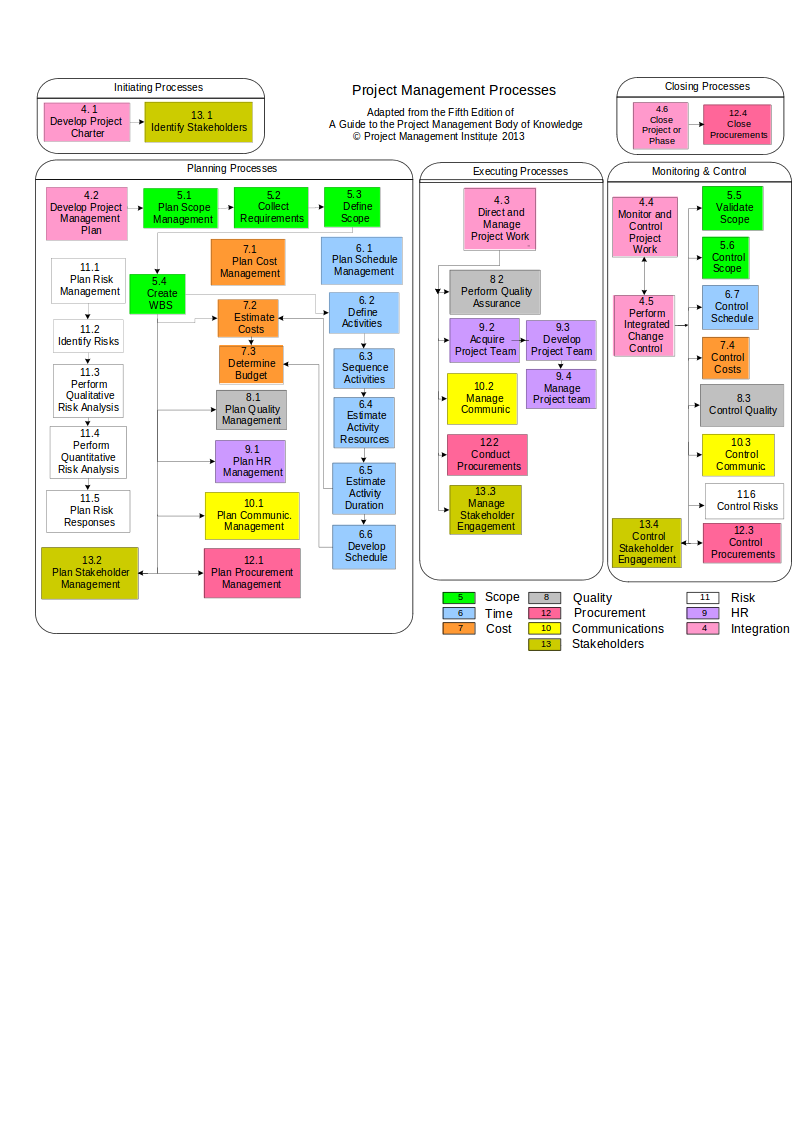
\includegraphics[scale=0.3]{mapping}
\end{figure}
\end{frame}

%---------------------------------------------------------
\begin{frame}
\frametitle{Restricting the Focus}
Unfortnately, we cannot focus on every task in the \textbf{Planning} process group in a single week. This week we will be looking at two knowledge areas: \textbf{Integration}, and \textbf{Scope}.

\begin{figure}
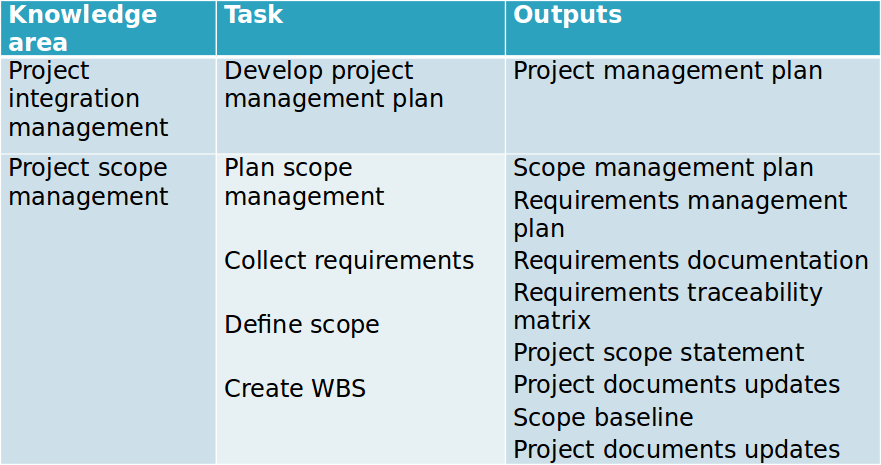
\includegraphics[scale=0.4]{planning_proc}
\caption{Our attention will be restricted to 2 knowledge areas}
\end{figure}
\end{frame}
%---------------------------------------------------------

\begin{frame}
\frametitle{Project Management Plan}
\vspace{-0.5cm}
\begin{figure}
\caption{The task of developing a project management plan is in the \textbf{Integration} knowledge area, and belongs to the \textbf{Planning} process group.}
\vspace{-0.8cm}
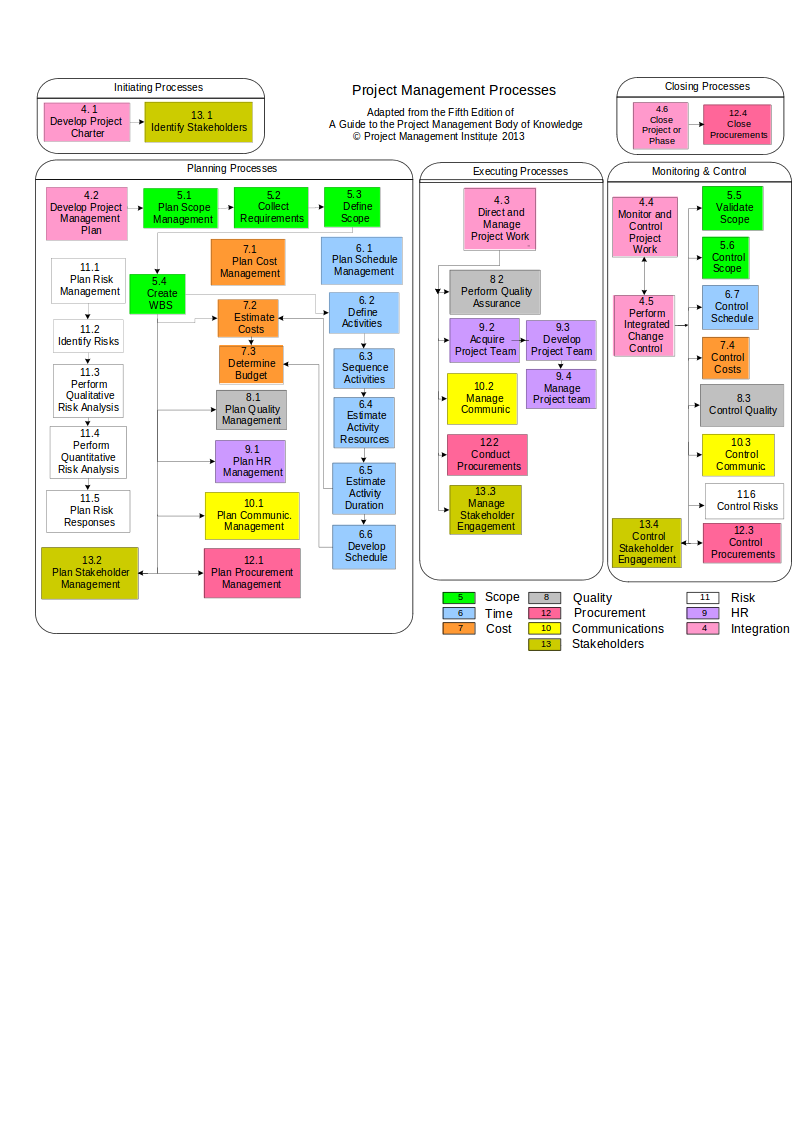
\includegraphics[scale=0.3]{mapping}
\end{figure}
\end{frame}
%---------------------------------------------------------

\begin{frame}
\frametitle{Project Management Plan}
\begin{block}{Definition: \textbf{Project Management Plan}}
A \textbf{project management plan} is a document used to coordinate all project planning documents and to help guide a project's execution and control
\end{block}

\begin{itemize}
\item Plans created in the other knowledge areas are subsidiary parts of the overall project management plan and provide more detailed information about that knowledge area
\item Project management plans facilitate communication among stakeholders and provide a \textbf{baseline} for progress measurement and project control
\end{itemize}

\begin{block}{Definition: \textbf{Baseline}}
A \textbf{baseline} is a starting point, a measurement, or an observation that is documented so that it can be used for future comparison
\end{block}
\end{frame}

%---------------------------------------------------------
\begin{frame}
\frametitle{Project Management Plans}
\textbf{Attributes of Project Management Plans}\\
\vspace{0.5cm}
\begin{itemize}
\item Project management plans should be dynamic, flexible, and receptive to change when the environment or project changes
\item Just as projects are unique, so are project plans.
\begin{itemize}
\item For a small project involving a few people over a couple of months, a project charter, team contract, scope statement, and Gantt chart might be the only project planning documents needed; there would not be a need for a separate project management plan
\item A large project involving 100 people over three years would benefit from having a detailed project management plan and separate plans for each knowledge area
\end{itemize}
\item It is important to tailor all planning documentation to fit the needs of specific projects
\end{itemize}
\end{frame}

%---------------------------------------------------------
\begin{frame}
\frametitle{Project Management Plans}
\begin{tcolorbox}
\textbf{Elements in Project Management Plans}
\begin{enumerate}
\item Introduction/Overview
\item Project Organisation
\item Management
\item Technical processes
\item Work to be performed
\item Schedule information
\item Budget information
\item References to other documents
\end{enumerate}
\end{tcolorbox}
\end{frame}

%---------------------------------------------------------
\begin{frame}
\frametitle{Project Management Plan}
\textbf{Sample Project Management Plan (Partial)}\\
\vspace{0.5cm}
\small
\textbf{Management:}
\begin{enumerate}
\item \textit{Management Review Process}: The project steering committee will meet at least monthly to provide inputs and review progress on this project.
\item \textit{Progress Measurement Process}: The project steering committee will review project progress during project review meetings, and they can also review information as needed by viewing reports on the enterprise project management software. Post project progress will also be measured to see if the project met its goals. These goals include reducing the training cost per employee by \$100/person/year and receiving positive results from survey participants on the effectiveness of the training.
\item \textit{Change Approval Process}: See Attachment 1 based on corporate standards.
\item \textit{Supplier Management Process}: See Attachment 2 based on corporate standards.
\end{enumerate}
\end{frame}

%---------------------------------------------------------
\begin{frame}
\frametitle{Project Management Plan}
\textbf{Sample Project Management Plan (Partial)}\\
\vspace{0.5cm}
\small
\textbf{Technical Processes:}
\begin{enumerate}
\item \textit{Enterprise Project Management Software}: All tasks, costs, resources, issues, and risks will be tracked for this project using our enterprise project management software. Data must be entered on a weekly basis, at a minimum, to provide timely information. 
\item \textit{Supplier Evaluation}: The project team will coordinate with the purchasing department to follow our standard procedures for selecting and working with suppliers. See Attachment 2 for corporate standards.
\end{enumerate}
\end{frame}

%---------------------------------------------------------

\begin{frame}
\frametitle{Plan Scope Mangement}
\vspace{-0.5cm}
\begin{figure}
\caption{The task of developing a scope management plan is in the \textbf{Scope} knowledge area, and belongs to the \textbf{Planning} process group.}
\vspace{-0.8cm}
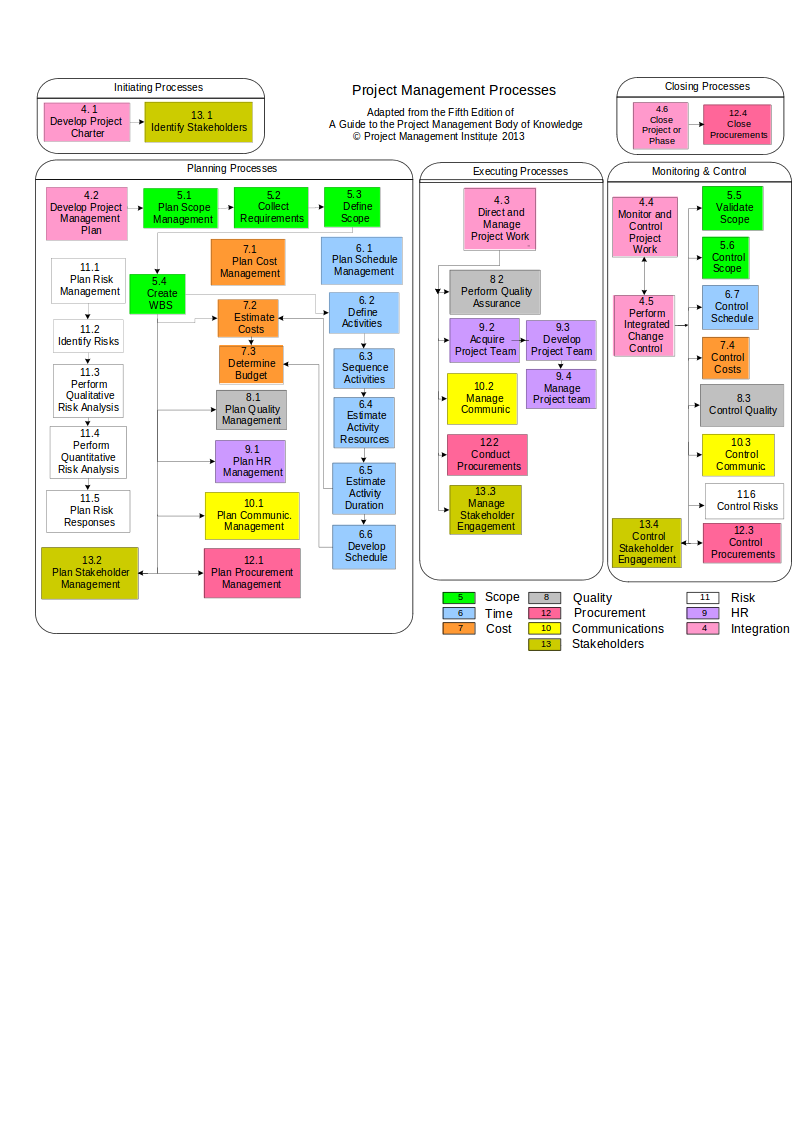
\includegraphics[scale=0.3]{mapping}
\end{figure}
\end{frame}

%---------------------------------------------------------

\begin{frame}
\frametitle{Plan Scope Management}
\begin{itemize}
\item The purpose of the plan scope management task is to determine how the project scope will be defined, validated, and controlled.
\vspace{0.5cm}
\item Project teams usually have several meetings with key stakeholders and experts to help them develop a \textbf{scope management plan} and \textbf{requirements management plan}.
\end{itemize}
\end{frame}

%---------------------------------------------------------

\begin{frame}
\frametitle{Plan Scope Management}
\begin{tcolorbox}
\textbf{Elements in a Requirements Management Plan}
\begin{enumerate}
\item Planning, tracking, and reporting requirements
\item Performing configuration management activities, such as initiating, analysing, tracking, and reporting changes to requirements
\item Prioritising requirements
\item Using product metrics
\item Tracing requirements
\end{enumerate}
\end{tcolorbox}

\end{frame}

%---------------------------------------------------------

\begin{frame}
\frametitle{Plan Scope Management}
\textbf{Sample Requirements Management Plan (Partial)}
\begin{figure}
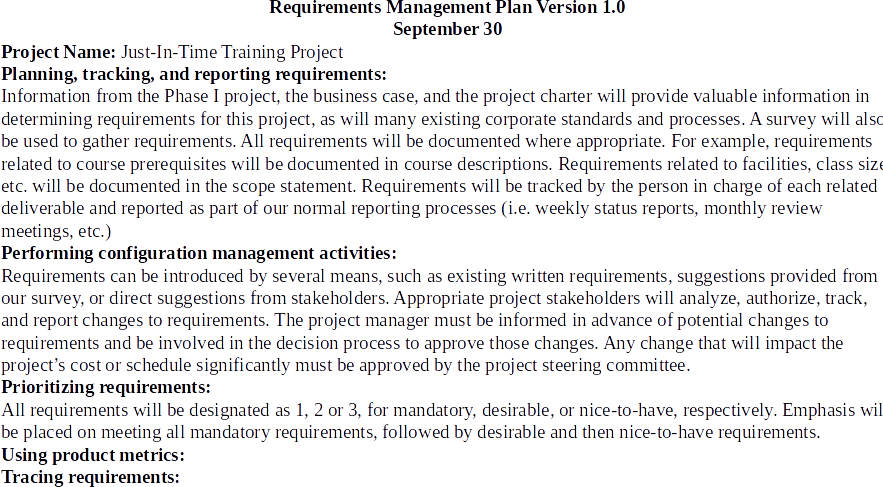
\includegraphics[scale=0.45]{req_man}
\vspace{-0.3cm}
\caption{An example of a requirements management plan}
\end{figure}
\end{frame}
%---------------------------------------------------------

\begin{frame}
\frametitle{Collecting Requirements}
\vspace{-0.5cm}
\begin{figure}
\caption{The task of developing a scope management plan is in the \textbf{Scope} knowledge area, and belongs to the \textbf{Planning} process group.}
\vspace{-0.8cm}
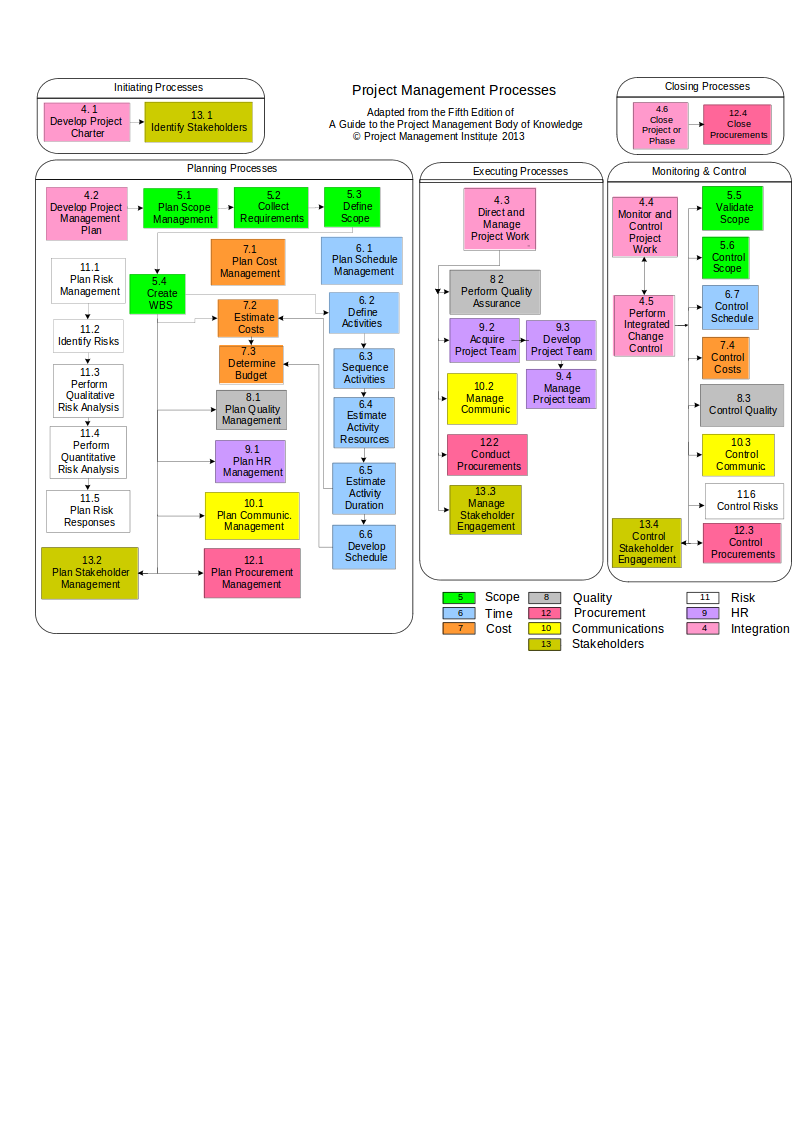
\includegraphics[scale=0.3]{mapping}
\end{figure}
\end{frame}

%---------------------------------------------------------

\begin{frame}
\frametitle{Collecting Requirements}
\vspace{0.5cm}
\begin{block}{Definition: \textbf{Requirements}}
The \textit{PMBOK Guide}, Fifth Edition, defines requirements as “conditions or capabilities that must be met by the project or present in the product, service, or result to satisfy an agreement or other formally imposed specification”
\end{block}
\vspace{0.3cm}
\begin{itemize}
\item A project’s size, complexity, importance, as well as other factors affect how much effort is spent on collecting requirements
\vspace{0.5cm}
\item Requirements must be documented in enough detail so that they can be measured during project execution
\end{itemize}
\end{frame}

%---------------------------------------------------------

\begin{frame}
\frametitle{Collecting Requirements}
\textbf{Outputs of Collecting Requirements}\\
\vspace{0.5cm}
The main output is a \textbf{requirements traceability matrix (RTM)}, which is a table that lists requirements, various attributes of each requirement, and the status of the requirements to ensure that all of them are addressed.
\vspace{0.3cm}
\begin{figure}
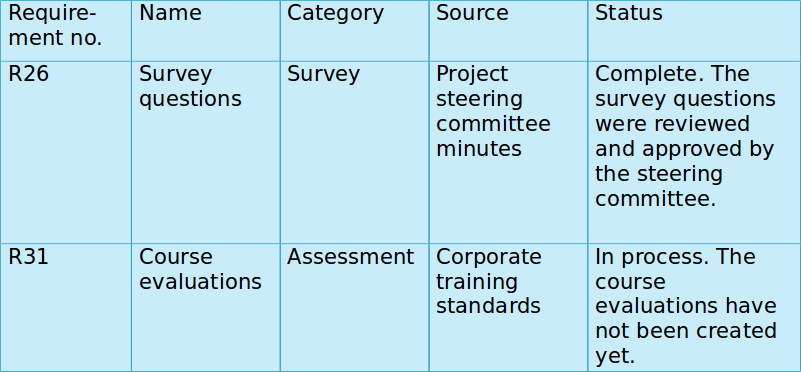
\includegraphics[scale=0.35]{requirements_mat}
\caption{An example of a requirements matrix.}
\end{figure}
\end{frame}
%---------------------------------------------------------

\begin{frame}
\frametitle{Define Scope}
\vspace{-0.5cm}
\begin{figure}
\caption{The task of defining the scope is in the \textbf{Scope} knowledge area, and belongs to the \textbf{Planning} process group.}
\vspace{-0.8cm}
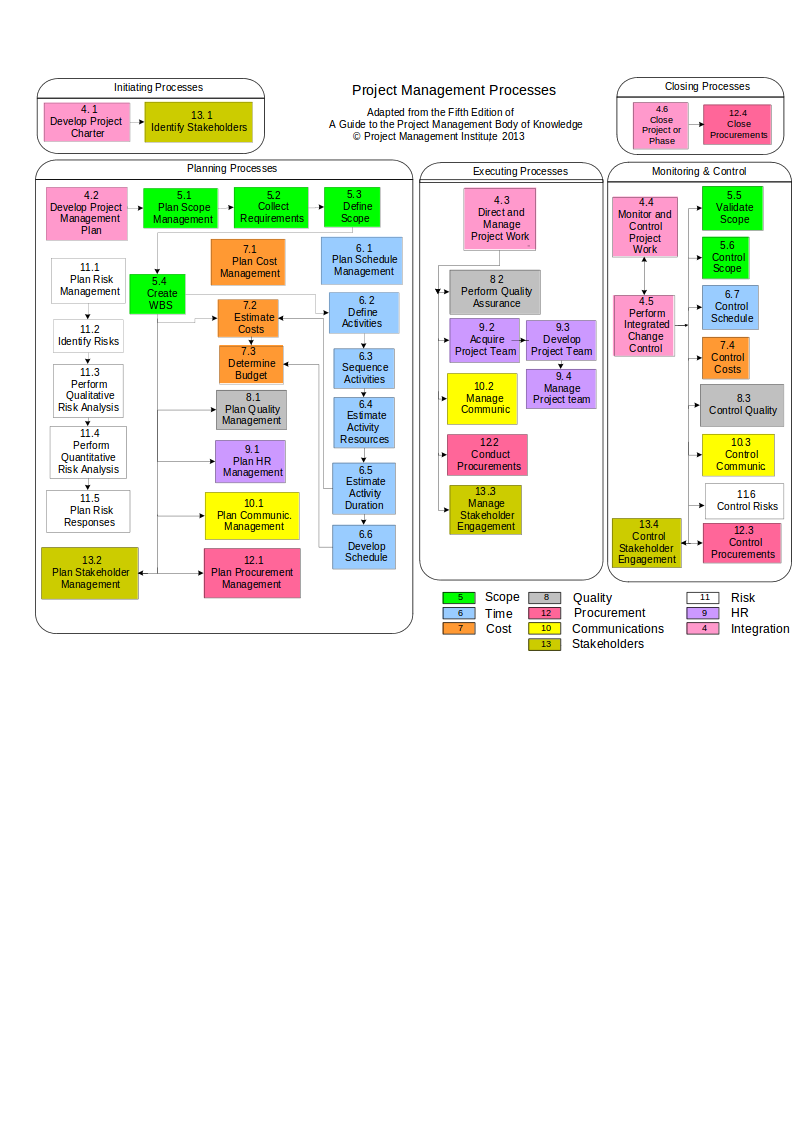
\includegraphics[scale=0.3]{mapping}
\end{figure}
\end{frame}

%---------------------------------------------------------

\begin{frame}
\frametitle{Define Scope}
\small
The purpose of the defining the scope is so:
\begin{itemize}
\item Estimates of time, cost, and resources can be made more accurate
\item A baseline can be clearly defined for effective performance management
\item Transparency is created surrounding work responsibilities - work that is not included in the scope should \underline{not} be done
\end{itemize}

The main output from this task is the \textbf{scope statement}. To effectively create this document, the following are required:
\begin{itemize}
\item Project charter
\item Requirements documentation
\item \textbf{Organisational process assets}

\begin{block}{Definition: \textbf{Orgaisational Process Assets}}
\textbf{Orgaisational Process Assets} are documents which include policies and procedures related to project management, past project files, and lessons learned from similar projects
\end{block}
\end{itemize}
\end{frame}

%---------------------------------------------------------

\begin{frame}
\frametitle{Define Scope}
\begin{tcolorbox}
\textbf{Elements in a Scope Statement}
\begin{enumerate}
\item Product scope description
\item Product user acceptance criteria
\item Detailed information on project deliverables
\item Project boundaries, constraints, and assumptions
\item Reference to all supporting documentation such as corporate policies, and product specifications
\end{enumerate}
\end{tcolorbox}
\end{frame}

%---------------------------------------------------------

\begin{frame}
\frametitle{Define Scope}
\textbf{Sample Scope Statement}
\begin{figure}
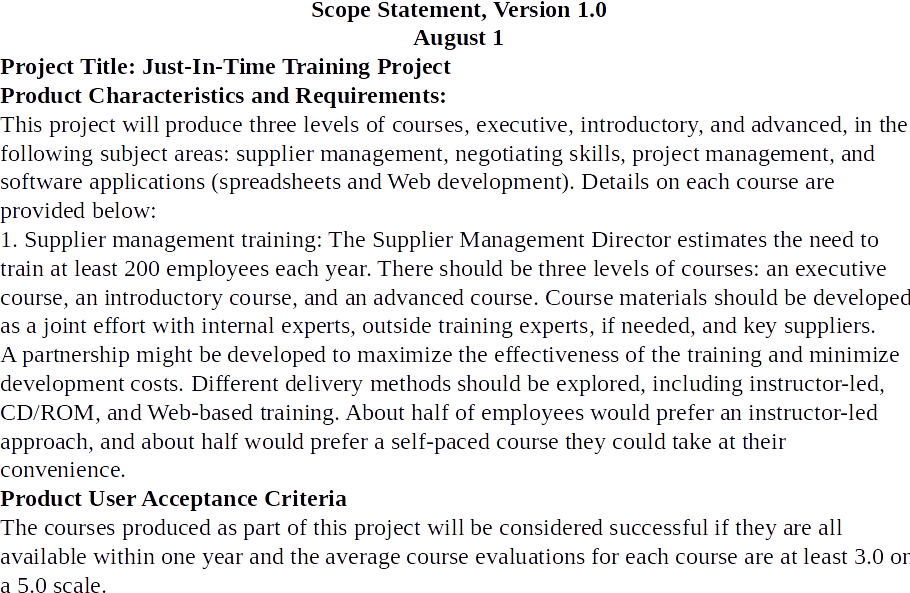
\includegraphics[scale=0.35]{scope_stat_1}
\vspace{-0.3cm}
\caption{An example of a scope statement}
\end{figure}
\end{frame}

%---------------------------------------------------------

\begin{frame}
\frametitle{Define Scope}
\textbf{Sample Scope Statement (Continued)}
\begin{figure}
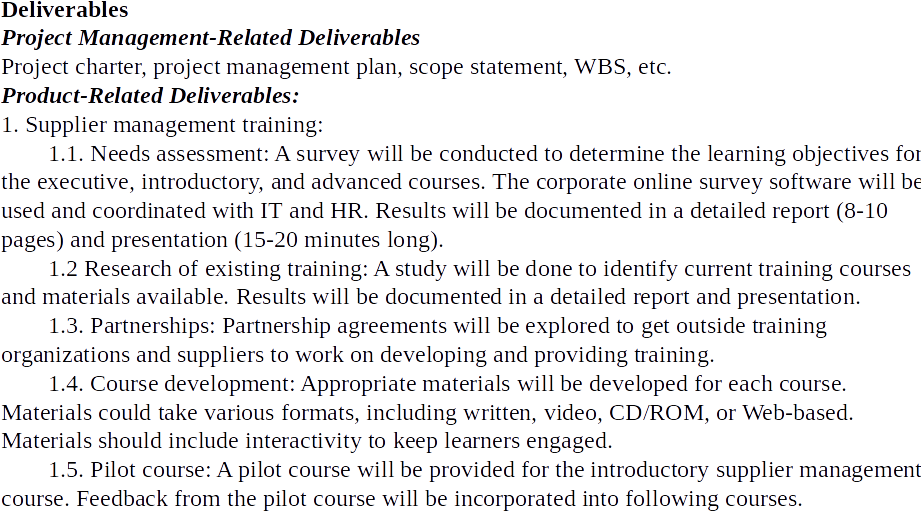
\includegraphics[scale=0.35]{scope_stat_2}

\caption{An example of a scope statement}
\end{figure}
\end{frame}

%---------------------------------------------------------

\begin{frame}
\frametitle{Define Scope}
\textbf{Keep Scope Information Current}
\vspace{0.5cm}
\begin{itemize}
\item The project team should update the project scope statement as new information becomes available
\item Name different iterations of the scope statement, for example Version 1.0, Version 2.0, etc
\item A good, up-to-date scope statement helps prevent scope creep, which is the tendency for project scope to continually increase.
\end{itemize}
\end{frame}

%---------------------------------------------------------

\begin{frame}
\frametitle{Creating the Work Breakdown Strucuture (WBS)}
\vspace{-0.5cm}
\begin{figure}
\caption{The task of creating the WBS is in the \textbf{Scope} knowledge area, and belongs to the \textbf{Planning} process group.}
\vspace{-0.8cm}
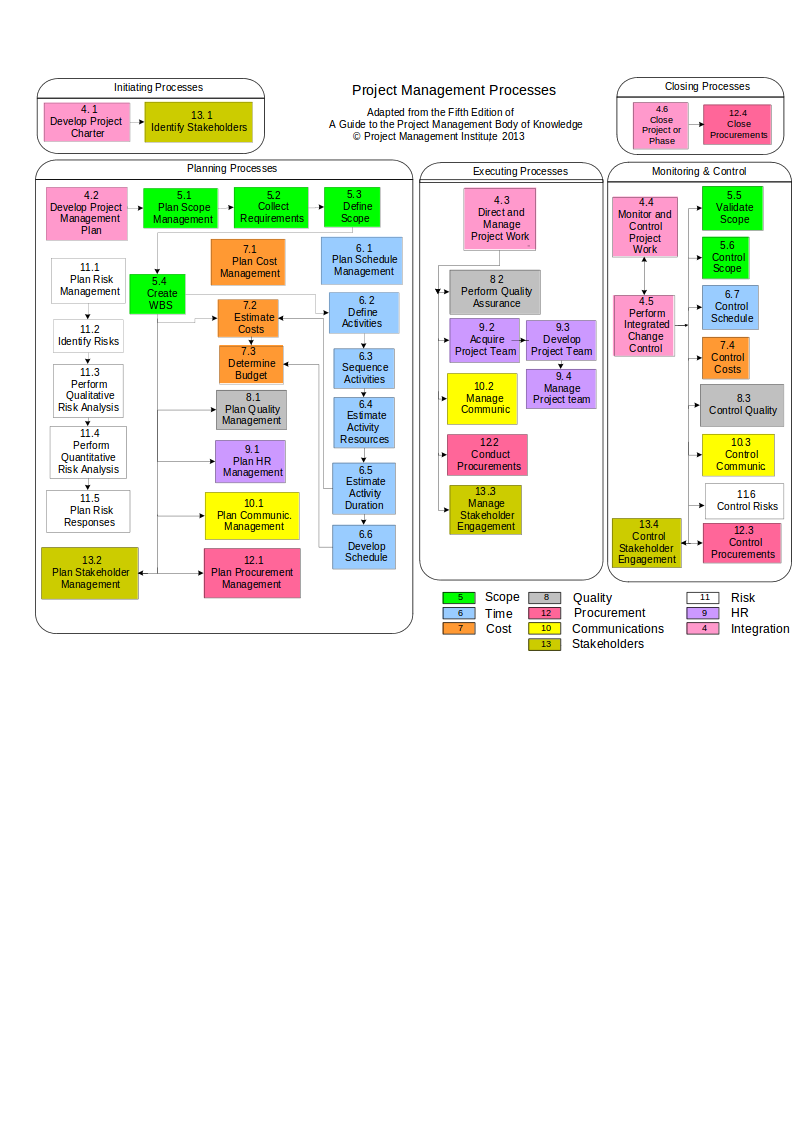
\includegraphics[scale=0.3]{mapping}
\end{figure}
\end{frame}

%---------------------------------------------------------

\begin{frame}
\frametitle{Creating the Work Breakdown Strucuture (WBS)}
\begin{block}{Definition: \textbf{Work Breakdown Structure (WBS)}}
A \textbf{WBS} is a deliverable-oriented grouping of the work involved in a project that defines the total scope of the project
\end{block}
A WBS is a document that breaks all the work required for the project into:
\begin{itemize}
\item discrete tasks; and
\item groups those tasks into a logical hierarchy with the lowest level being the \textbf{work package}
\end{itemize}

\begin{block}{Definition: \textbf{Work Package}}
A \textbf{work package} is a deliverable at the lowest level of the WBS, where it can be appropriately assigned to and managed by a single accountable person.
\end{block}
\end{frame}

%---------------------------------------------------------

\begin{frame}
\frametitle{Creating the Work Breakdown Strucuture (WBS)}
\textbf{The Importance of a Good WBS}
\vspace{0.25cm}
\small
\begin{itemize} 
\item Foundational document in project management because it provides the basis for planning and managing project schedules, costs, resources, and changes
\item The WBS contains 100\% of the deliverables (often called “work”) of the project
\item Often the WBS is shown in two different forms: \textbf{graphical (chart) form}, or \textbf{tabular (list) form}.
\end{itemize}
\vspace{0.5cm}
\textbf{WBS Attributes}\\
\vspace{0.25cm}
\small A WBS shows:
\begin{itemize}
\item the various elements of the project, 
\item how work is distributed between project elements,
\item how the cost or budget is distributed between project elements
\item how the larger elements are subdivided into smaller ones
\end{itemize}
\end{frame}

%---------------------------------------------------------

\begin{frame}
\frametitle{Creating the Work Breakdown Strucuture (WBS)}
\textbf{WBS Attributes}
\begin{figure}
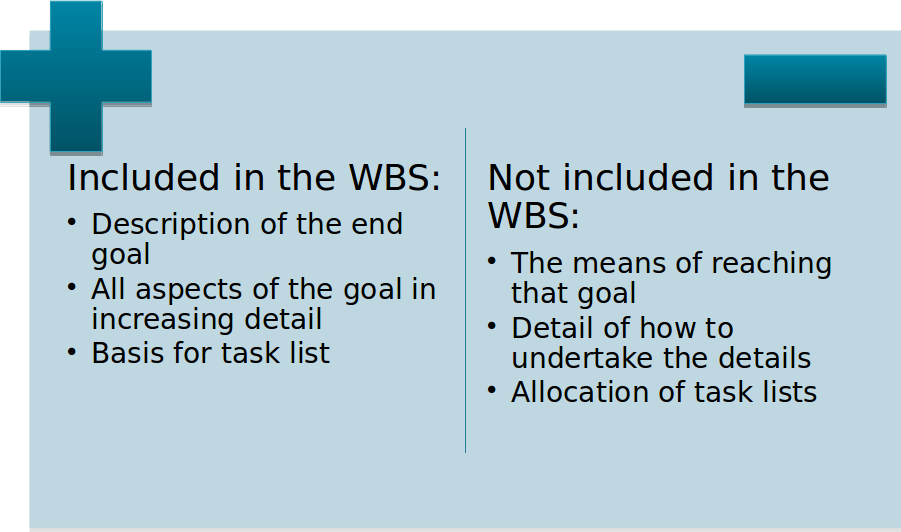
\includegraphics[scale=0.45]{wbs_att}
\end{figure}
\end{frame}

%---------------------------------------------------------

\begin{frame}
\frametitle{Creating the Work Breakdown Strucuture (WBS)}
\textbf{An Example of a Graphical WBS}
\begin{figure}
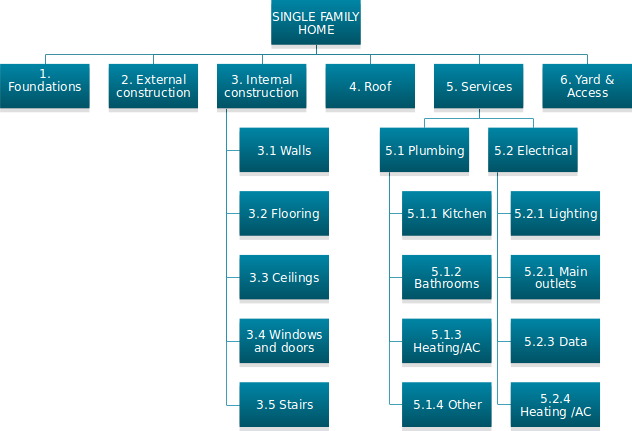
\includegraphics[scale=0.5]{wbs_graph}
\caption{An example of a WBS in graphical form.}
\end{figure}
\end{frame}

%---------------------------------------------------------

\begin{frame}
\frametitle{Creating the Work Breakdown Strucuture (WBS)}
\textbf{WBS PMI Numbering}
\begin{figure}
\boxed{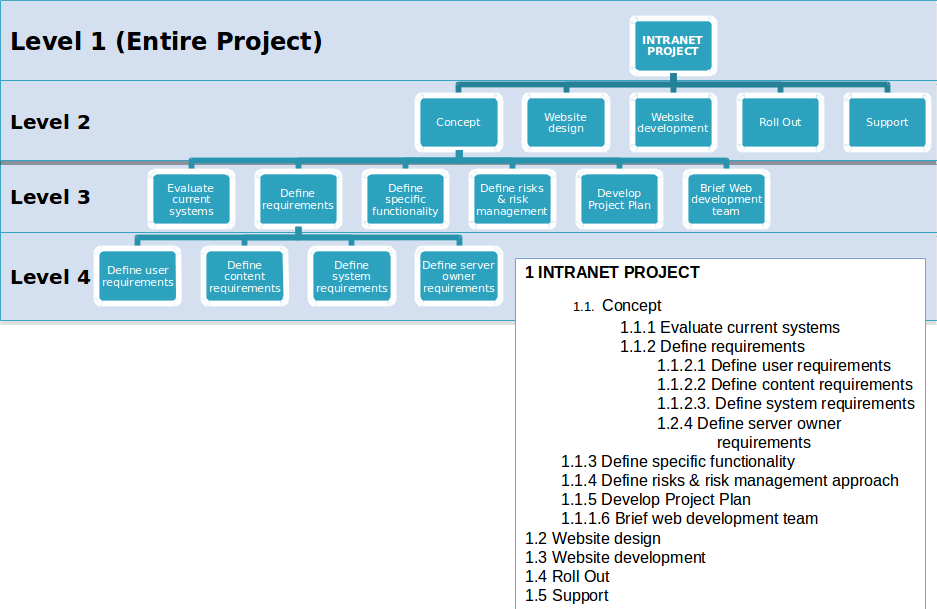
\includegraphics[scale=0.35]{wbs_pmi}}
\end{figure}
\end{frame}

%---------------------------------------------------------

\begin{frame}
\frametitle{Creating the Work Breakdown Strucuture (WBS)}
\textbf{WBS MS Project Numbering}
\begin{figure}
\boxed{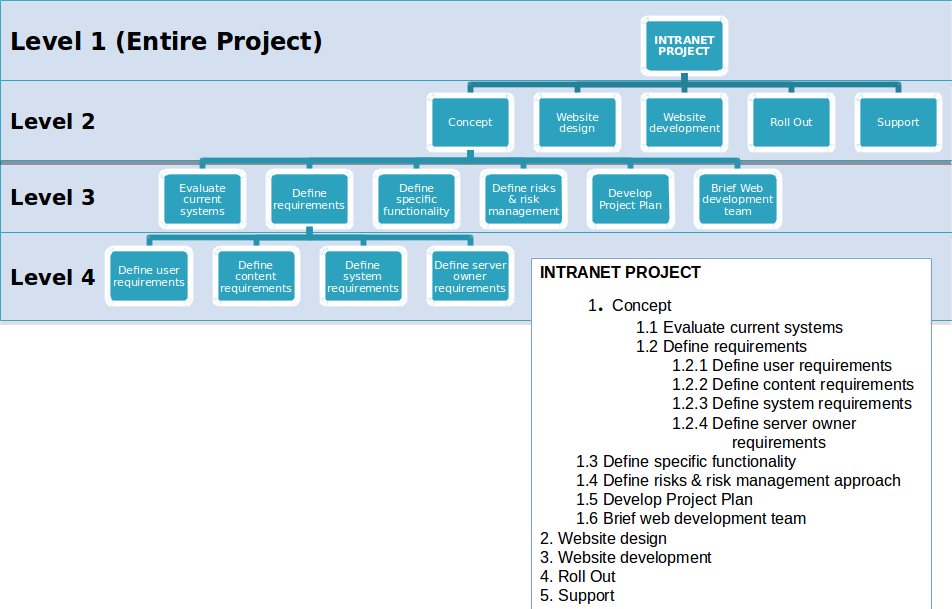
\includegraphics[scale=0.35]{wbs_ms}}
\end{figure}
\end{frame}

%---------------------------------------------------------

\begin{frame}
\frametitle{Creating the Work Breakdown Strucuture (WBS)}
\textbf{Best Practice for Creating a WBS}
\vspace{0.5cm}
\begin{itemize}
\item If you look closely at the WBS example shown you will notice that there are no verbs, as verbs represent action, and a WBS is not about action, but rather about deliverables.
\vspace{0.3cm}
\item It is incorrect to show activities on the WBS, according to PMI, so try to consistently use deliverables on your WBS. Activities should be shown on the schedule and not on the WBS itself.
\vspace{0.3cm}
\item Several project management software packages use the WBS to create the activities, which may also cause some confusion. Use your judgement to decide the best way to create a WBS and the wording on it.
\end{itemize}
\end{frame}
%---------------------------------------------------------

\begin{frame}
\frametitle{Creating the Work Breakdown Strucuture (WBS)}
\textbf{How to Create a Good WBS}
\vspace{0.5cm}
\begin{itemize}
\item It is difficult to create a good WBS
\vspace{0.2cm}
\item The project manager and the project team must decide as a group how to organise the work and how many levels to include in the WBS
\vspace{0.2cm}
\item It is often better to focus on getting the top levels of the WBS done well to avoid being distracted by too much detail
\vspace{0.2cm}
\item Many people confuse tasks on a WBS with specifications or think it must reflect a sequential list of steps
\vspace{0.2cm}
\item You should focus on what work needs to be delivered, not when or exactly how it will be done
\end{itemize}
\end{frame}

%---------------------------------------------------------

\begin{frame}
\frametitle{Creating the Work Breakdown Strucuture (WBS)}
\textbf{Approaches to Developing a WBS}
\begin{figure}
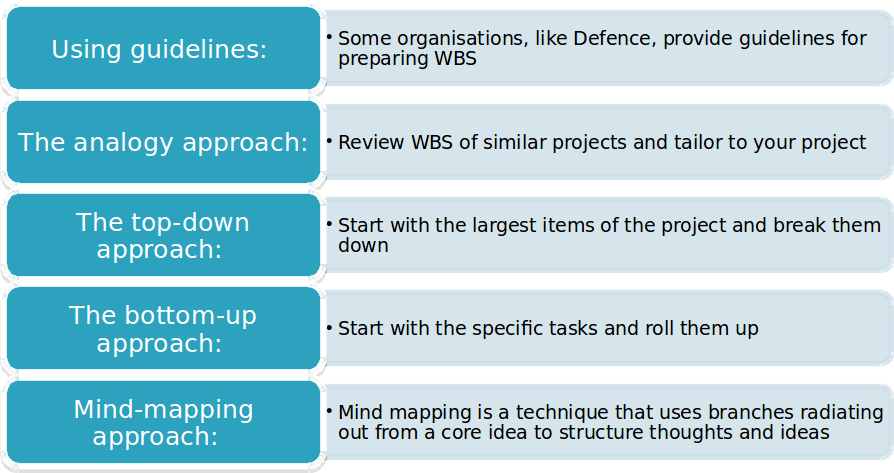
\includegraphics[scale=0.5]{wbs_approaches}
\end{figure}
\end{frame}

%---------------------------------------------------------

\begin{frame}
\frametitle{Creating the Work Breakdown Strucuture (WBS)}
\textbf{Sample Mindmapping Technique for Creating a WBS}
\vspace{0.5cm}
\begin{figure}
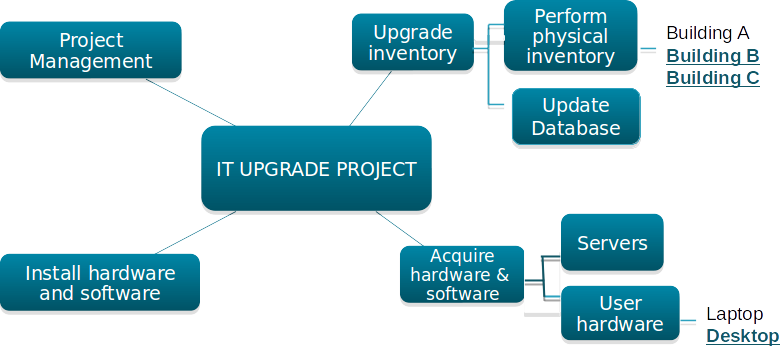
\includegraphics[scale=0.5]{mindmap_wbs}
\end{figure}
\end{frame}

%---------------------------------------------------------

\begin{frame}
\frametitle{Creating the Work Breakdown Strucuture (WBS)}
\textbf{Gantt Chart with WBS Generated from Mind Map}
\begin{columns}
\column{0.45\textwidth}
\begin{figure}
\boxed{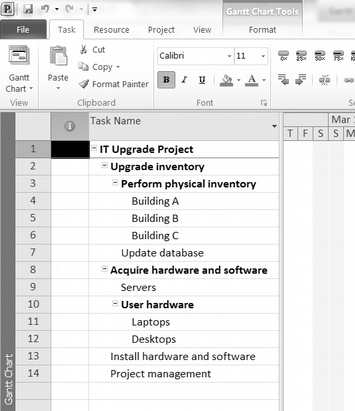
\includegraphics[height=5cm]{mindview_gantt}}
\caption{Gantt chart from mindmap with Mindview software}
\end{figure}
\column{0.5\textwidth}
\begin{figure}
\boxed{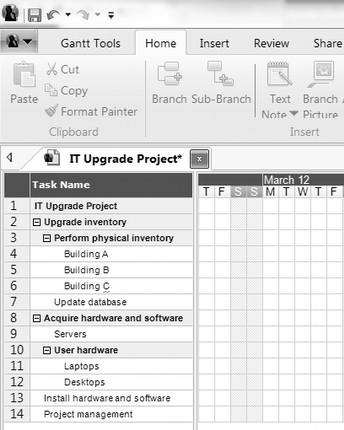
\includegraphics[height=5cm]{msproject_gantt}}
\caption{Gantt chart from mindmap with MS Project software}
\end{figure}
\end{columns}
\end{frame}

%---------------------------------------------------------

\begin{frame}
\frametitle{Creating the Work Breakdown Strucuture (WBS)}
\textbf{Creating the WBS Dictionary}
\vspace{0.25cm}
\begin{block}{Definintion: \textbf{WBS Dictionary}}
A \textbf{WBS dictionary} is a document that describes each WBS task in detail.
\end{block}
\vspace{0.25cm}
The format of the WBS dictionary can vary based on the projects needs:
\begin{itemize}
\item The WBS dictionary may just be a short paragraph that describes each \textbf{work package}.
\item If the project is complex then an entire page or more might be required to describe the work package.
\end{itemize}
\vspace{0.2cm}
Some common elements that are included in the work package description:
\vspace{-0.1cm}
\begin{itemize}
\item The responsible person or organisation;
\item The resource requirements;
\item The estimated costs of the work package;
\end{itemize}
\end{frame}

%---------------------------------------------------------

\begin{frame}
\frametitle{Creating the Work Breakdown Strucuture (WBS)}
\textbf{Sample of a WBS Dictionary Entry}
\vspace{0.5cm}
\begin{figure}
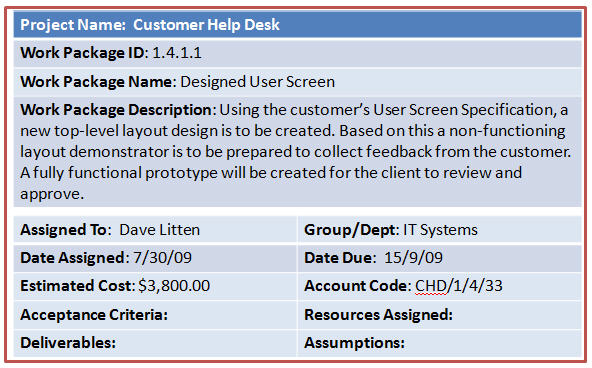
\includegraphics[scale=0.5]{wbsdictionary}
\end{figure}
\end{frame}

%---------------------------------------------------------

\begin{frame}
\begin{center}
\huge The End
\end{center}
\end{frame}

\end{document} 